\chapter{Implementation}

This chapter shares some notes of the implementation with future developers. 

\section{Comprehensive search}
Given a covariate $X_i$ and a particular cut value $c$, there are two
treatment recommendations. 
\begin{description}
\item[Recommendation 1 ($R_1$):] Give treatment 1 if $X_i < c$ and treatment 0
  otherwise.
\item[Recommendation 2 ($R_2$):] Give treatment 1 if $X_i \geq c$ and treatment 0
  otherwise. 
\end{description}
In other words, $R_1=I_{X_i < c}$ and $R_2=I_{X_i \geq c}$. In the implementation,
the bitmask $I_{X_i<c}$ for each cut is saved. One way to implement the search is

\begin{lstlisting}
// Depth one 
double v[2] = {0.0}; 
for (size_t i = 0; i < N; ++i) {
  v[0] += y[i] * (a[i] == m[i]);       // X < c
  v[1] += y[i] * (a[i] == 1 - m[i]);   // X >= c
}

// Depth two 
double v[4] = {0.0}; 
for (size_t i = 0; i < N; ++i) {
  // X1 < c1 and X2 < c2
  v[0] += y[i] * (a[i] == m1[i]) * (a[i] == m2[i]); 
  
  // X1 < c1 and X2 >= c2
  v[1] += y[i] * (a[i] == m1[i]) * (a[i] == 1 - m2[i]);

  // X1 >= c1 and X2 < c2
  v[2] += y[i] * (a[i] == 1 - m1[i]) * (a[i] == m2[i]);

  // X1 >= c1 and X2 >= c2 
  v[3] += y[i] * (a[i] == 1 - m1[i]) * (a[i] == 1 - m2[i]);
}
\end{lstlisting}
As the depth of search increases, this implementation becomes more cumbersome.
However, if the package is to be deployed on GPUs, the above implementation
can be revised to utilize vectorization. Currently, the package is intended to
run on multicore computers, and the computation is organized differently which
we explain next. 

\begin{figure}[h]
  \centering
  \caption{Demonstration of depth one search}
  \label{fig:depth1}
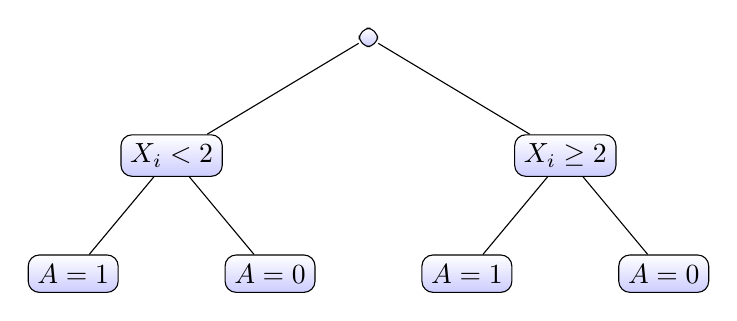
\begin{tikzpicture}[
  level/.style={sibling distance = 5cm/#1,
    level distance = 1.5cm},
  every node/.style = {shape=rectangle, rounded corners,
    draw, align=center,
    top color=white, bottom color=blue!20}
  ]
  \node {} % Root
  % left child
  child { node {$X_i <2$}
    child { node {$A=1$} }
    child { node {$A=0$} }
  }
  % right child
  child { node {$X_i \geq 2$}
    child { node {$A=1$} }
    child { node {$A=0$} }
  };
\end{tikzpicture}
\end{figure}

Consider the depth one case shown in Figure~\ref{fig:depth1}. Recall
that the bitmask of $X_i < 2$ is stored as a vector. For each sample
$j$ being processed, there are four combinations depending on the
value of $A_j$ and the bitmask $X_{ij} < c$. This means, the
corresponding $Y_j$ can be sorted into four buckets. For instance, the
far left bucket corresponds to $X_{ij} < c$ and $A_j=1$ and can
therefore be indexed as bucket 3 (=$(11)_2$). The far right bucket can
be indexed as bucket 0 ($=(00)_2$) and $B_k$, $k=0,1,2,3$ denote the
sets of $Y_j$ in each bucket and $S_{T_0}$ is a set of $Y_j$ where $j$
satisfies $A_j=0$.  Notice that the sets have the following
relationship,
\[B_3 - B_2 + T_0 
=  \{A = 1 \cap X_i < 2\} - \{A = 0 \cap X_i < 2\} + \{A = 0\}
= \{A = 1 \cap X _i< 2\} + \{A = 0 \cap X_i \geq 2\}
\]
%
Let $T_0$ be
\[
T_0 = \sum_{j:A_j = 0} Y_j
\]
If the treatment recommendation is $I(X_i < 2)$, the recommendation is
treatment 0, the value of $\sum_j I\{A_j=I(X_{ij}<2)\}Y_j$ can be
calculated as the sum of $Y_j$ where $j \in \{B_3 - B_2 + T_0\}$.
Similarly, one can verify that if the treatment recommendation is
$I(X_i \geq 2)$, the sum can be based on the $Y_j$ where $j \in \{B_1
- B_0 + T_0\}$.

We may notice that the $\{B_3 - B_2 + T_0\}=\{B_3+B_0\}$ and $\{B_1 -
B_0 + T_0\}=\{B_2+B_1\}$. Therefore, we do not need to calculate $T_i$
in this example. However, when the depth is equal to 3, the above
calculation will be more efficient.

